\addcontentsline{toc}{chapter}{Занятие 7. $L_2$ теория}
\chapter*{Занятие 7. $L_2$ теория}

\addcontentsline{toc}{section}{Контрольные вопросы и задания}
\section*{Контрольные вопросы и задания}

\subsubsection*{Приведите опредедение непрерывного в среднем квадратическом случайного процесса.}

$ \xi $ непрерывен в среднем квадратическом в точке $t_0$, если
$$ \xi \left( t \right) \overset{L_2}{ \to }
  \xi \left( t_0 \right) $$
при $t \to t_0$,
то есть $M \left[ \xi \left( t \right) - \xi \left( t_0 \right) \right]^2 \to 0, \, t \to t_0$.

Случайный процесс $ \xi $ непрерывен в среднем квадратическом на $T$,
если $ \xi $ непрерывен в среднем квадратическом в каждой точке $t_0 \in T$.

\subsubsection*{Как определяются производная случайного процесса, интеграл случайного процесса?}

$ \xi $ дифференцируем в среднем квадратическом в точке $t_0$, если
$$ \exists L_2-\lim \limits_{t \to t_0}
    \frac{ \xi \left(t \right) - \xi \left( t_0 \right) }{t - t_0} =
  \xi' \left( t_0 \right).$$

Случайный процесс $ \xi $ интегрируем в среднем квадратическом на отрезке $ \left[ a, b \right] $,
если
$$ \exists L_2-\lim \limits_{ \left| \pi \right| \to 0}
    \sum \limits_{k = 0}^{n - 1} \xi \left( t_k \right) \Delta t_k,$$
где $ \pi $ --- разбиение: $a = t_0 < \dotsc < t_n = b$.

Модуль разбиения --- это максимумальная разность между соседними точками.

\subsubsection*{Как изменяются характеристики случайного процесса при дифференцировании,
                интегрировании?}

$ \xi \in L_2 \, : \, M \left| \xi \right|^2 < \infty, \,
  \left( \xi, \eta \right) = M \xi \overline{ \eta }, \,
  \left( \xi, \xi \right) = M \left| \xi \right|^2$.

\subsubsection*{Приведите условия непрерывности, дифференцируемости,
                интегрируемости случайного процесса в терминах его ковариационной функции.}

$ \xi $ непрерывен в среднем квадратическом на интервале $T$ тогда и только тогда,
когда $m \in C \left( T \right), \, K \in C \left( T \times T \right) $.

Случайный процесс $ \xi $ дифференцируем в среднем квадратическои в точке $t_0$
тогда и только тогда, когда $m$ дифференцируема в точке $t_0$ и
$$ \exists \lim \limits_{s, t \to t_0}
    \frac{K \left( t, s \right) - K \left( t, t_0 \right) - K \left( t_0, s \right) + K \left( t_0, t_0 \right) }{ \left( s - t_0 \right) \left( t - t_0 \right) }.$$

Непрерывный в среднем квадратическом на отрезке $ \left[ a, b \right] $ процесс $ \xi $
интегрируем в среднем квадратическом на этом отрезке.

\addcontentsline{toc}{section}{Аудиторные задачи}
\section*{Аудиторные задачи}

\subsubsection*{7.2}

\textit{Задание.}
Пусть $ \zeta_1, \dotsc, \zeta_n$ --- интегрируемые с квадратом случайные величины.
Докажите, что случайный процесс
$$ \xi \left( t \right) =
  \sum \limits_{k = 1}^n \zeta_k e^{kt}$$
имеет производную в среднем квадратическом и найдите её.

\textit{Решение.}
$ \zeta_1, \dotsc, \zeta_n \in L_2$, то есть есть $n$ величин, и процесс определяется как
$$ \xi \left( t \right) =
  \sum \limits_{k = 1}^n \zeta_l e^{kt}.$$
Нужно проверить, что этот процесс дифференцируем и найти его производную в $L_2$.

Время $t$ входит только в экспоненту, которую мы умеем дифференцировать.
Нужно проверить, что
$$ \left \Vert
    \frac{ \xi \left( t \right) - \xi \left( t_0 \right) }{t - t_0} -
    \sum \limits_{k = 1}^n \zeta_k ke^{kt_0} \right \Vert \to
  0,$$
когда $t \to t_0$.

Будем это проверять.
Можно $ \xi \left( t \right) $ расписать.

$ \xi \left( t \right) $ --- это сумма
$$ \left \Vert
    \frac{ \xi \left( t \right) - \xi \left( t_0 \right) }{t - t_0} -
    \sum \limits_{k = 1}^n \zeta_k k e^{kt_0} \right \Vert =
  \left \Vert
    \frac{ \sum \limits_{k = 1}^n \zeta_k e^{kt} - \sum \limits_{k = 1}^n \zeta_k e^{kt_0}}{t - t_0} -
    \sum \limits_{k = 1}^n \zeta_k ke^{kt_0} \right \Vert =$$
Во всех слагаемых есть сумма и $ \zeta_k$.
Так что приведём подобные, и будет одна сумма
$$= \left \Vert
    \sum \limits_{k = 1}^n \zeta_k \left( \frac{e^{kt} - e^{kt_0}}{t - t_0} - ke^{kt_0} \right)
  \right \Vert \leq$$
Первое слагаемое в скобках стремится к производной, а второе и есть производная.
Их разность стремится к нулю.
Используем неравенство треугольника
$$ \leq \sum \limits_{k = 1}^n
  \left \Vert \zeta_k \left( \frac{e^{kt} - e^{kt_0}}{t - t_0} - ke^{kt_0} \right) \right \Vert =$$
С помощью свойства
$ \left \Vert \alpha \xi \right \Vert \leq
  \left| \alpha \right| \cdot \left \Vert \xi \right \Vert $
коэффициент выносится из нормы
$$= \sum \limits_{k = 1}^n
    \left| \frac{e^{kt} - e^{kt_0}}{t - t_0} - ke^{kt_0} \right| \cdot
    \left \Vert \zeta_k \right \Vert \to$$
Под модулем стоят числа, которые сходятся к нулю, под нормой --- числа
$$ \to 0.$$

\subsubsection*{7.3}

\textit{Задание.}
Пусть $ \left\{ W \left( t \right), \, t \geq 0 \right\} $ --- винеровский процесс.
Докажите, что случайный процесс
$$ \left\{ \eta \left( t \right) = \int \limits_0^t W \left( s \right) ds, \, t \geq 0 \right\} $$
являюется дифференцируемым в среднем квадратическом и что
$$ \eta' \left( t \right) =
  W \left( t \right) $$
для произвольного $t \geq 0$.

\textit{Решение.}
Дифференцируем интеграл по верхнему пределу.

Должна получиться подинтегральная функция.
Нужно проверить, что
$$ \frac{ \eta \left( t \right) - \eta \left( t_0 \right) }{t - t_0} \overset{L_2}{ \to }
  W \left( t_) \right).$$

Проверяем.
Вместо $ \eta $ подставляем интеграл
$$M \left[
    \frac{ \eta \left( t \right) - \eta \left( t_0 \right) }{t - t_0} - W \left( t_0 \right)
  \right]^2 =
  M \left[
    \frac{ \int \limits_0^t W \left( s \right) ds - \int \limits_0^{t_0} W \left( s \right) ds}{t - t_0} -
    W \left( t_0 \right)
  \right]^2 =$$
Разность интегралов --- это интеграл от $t_0$ до $t$.
Так что
$$= M \left[
    \frac{\int \limits_{t_0}^t W \left( s \right) ds}{t - t_0} - W \left( t_0 \right)
  \right]^2 =$$
Случайную величину $W \left( t_0 \right) $ можно внести под интеграл,
потому что он не зависит от $s$.
Знаменатель вынесем из-под интеграла
$$= M \left\{
    \int \limits_{t_0}^t \left[
      W \left( s \right) - W \left( t_0 \right)
    \right] ds
  \right\}^2 \cdot
  \frac{1}{ \left( t - t_0 \right)^2} =$$
Найдём дисперсию
$$D \int \limits_a^b \xi \left( s \right) ds =
  cov \left(
    \int \limits_a^b \xi \left( s \right) ds, \int \limits_a^b \xi \left( r \right) dr
  \right).$$
Ковариация --- это линейная функция, оба интеграла выносятся
$$cov \left(
    \int \limits_a^b \xi \left( s \right) ds, \int \limits_a^b \xi \left( r \right) dr
  \right) =
  \int \limits_a^b \int \limits_a^b
    cov \left[ \xi \left( s \right), \xi \left( t \right) \right]
  dsdr.$$
Тогда
$$= \frac{1}{ \left( t - t_0 \right)^2} \int \limits_{t_0}^t \int \limits_{t_0}^t cov \left[
    W \left( s \right) - W \left( t_0 \right), W \left( r \right) - W \left( t_0 \right) \right]
  dsdr =$$
Ковариацию винеровского процесса мы знаем
$$= \int \limits_{t_0}^t \int \limits_{t_0}^t \left[
    \min \left( s, r \right) - t_0 - t_0 + t_0 \right] dsdr \cdot
  \frac{1}{ \left( t - t_0 \right)^2} =$$
Одинаковые слагаемые с разными знаками уничножаются
$$= \int \limits_{t_0}^t \int \limits_{t_0}^t
    \left[ \min \left( s, r \right) - t_0 \right] dsdr \cdot
  \frac{1}{ \left( t - t_0 \right)^2} \leq
  \int \limits_{t_0}^t \int \limits_{t_0}^t \left( t - t_0 \right) dsdr \cdot
  \frac{1}{ \left( t - t_0 \right)^2} =$$
Величина $t - t_0 = const$, она вносится
$$= t - t_0 \to
  0.$$
Это и надо было проверить.

\subsubsection*{7.4}

\textit{Задание.}
Пусть $ \left\{ W \left( t \right), \, t \geq 0 \right\} $ --- винеровский процесс.
Докажите существование интеграла в среднем квадратическом
$$ \int \limits_0^{ \infty } e^{-t} W \left( t \right) dt =
  L_2-\lim \limits_{T \to + \infty } \int \limits_0^T e^{-t} W \left( t \right) dt$$
и найдите его распределение.

\textit{Решение.}
Рассматриваются интегралы
$$ \int \limits_0^T e^{-t} W \left( t \right) dt.$$
Нужно доказать, что у этих интегралов есть предел, то есть
$$ \int \limits_0^T e^{-t} W \left( t \right) dt \overset{L_2, \, T \to \infty }{ \to }?$$

Что нужно проверять, чтобы доказать, что этот интеграл сходится?
Надо брать математическое ожидание разностей в квадрате.
Предела мы не знаем.

Гильбертово пространство обладает свойством полноты
$$ \xi_n \overset{L_2, \, n \to \infty }{ \to }
  \xi$$
тогда и только тогда, когда $ \left\{ \xi_n \right\} $ фундаментальная, то есть
$$M \left( \xi_n - \xi_m \right)^3 \overset{n, m \to \infty }{ \to }
  0.$$

Предположим, что $T_1 < T_2$.
Из полноты следует, что нам достаточно проверить такое
$$M \left[
    \int \limits_0^{T_1} e^{-t} W \left( t \right) dt -
    \int \limits_0^{T_2} e^{-t} W \left( t \right) dt \right]^2 =
  M \left[ \int \limits_{T_1}^{T_2} e^{-t} W \left( t \right) dt \right]^2 =$$
Это двойной интеграл от ковариации
$$= \int \limits_{T_1}^{T_2} \int \limits_{T_1}^{T_2}
    cov \left[ e^{-t} W \left( t \right), e^{-s} W \left( s \right) \right] dtds =
  \int \limits_{T_1}^{T_2} \int \limits_{T_1}^{T_2}
    e^{-t-s} \min \left( t, s \right) dtds =$$
Нужно проверить, что это выражение стремится к нулю, когда $T_1, T_2 \to \infty $.
Распишем для всех случаев
$$= \int \limits_{T_1}^{T_2} \left( \int \limits_{T_1}^s e^{-t-s} tdt \right) ds +
  \int \limits_{T_1}^{T_2} \left( \int \limits_s^{T_2} e^{-t-s} sdt \right) ds \leq $$
Пусть $t < s$.
Тогда
$$ \leq \int \limits_{T_1}^{T_2} \left( \int \limits_{T_1}^s e^{-t-s} sdt \right) ds +
  \int \limits_{T_1}^{T_2} \left( \int \limits_s^{T_2} e^{-t-s} sdt \right) ds =
  \int \limits_{T_1}^{T_2} \int \limits_{T_1}^{T_2} e^{-s} e^{-t} sdtds =$$
Интегрируем по $y$, получаем
$$= \int \limits_{T_1}^{T_2} se^{-s} ds \int \limits_{T_1}^{T_2} e^{-t} dt =
  \int \limits_{T_1}^{T_2} se^{-s} ds \cdot \left( e^{-T_2} - e^{-T_1} \right) =$$
Берём интеграл по частям
$$= \left( e^{-T_2} - e^{-T_1} \right)
  \left( \left. -e^{-s} s \right|_{T_1}^{T_2} - \left. e^{-s} \right|_{T1}^{T_2} \right) =$$
Подставим пределы интегрирования
$$= \left( e^{-T_2} - e^{-T_1} \right)
  \left( -T_2 e^{-T_2} + T_1 e^{-T_1} - e^{-T_2} + e^{-T_1} \right)
  \overset{T_1, T_2 \to \infty }{ \to } 0,$$
Так как каждое слагаемое стремится к нулю,
то есть мы посчитали расстояние между двумя интегралами и показали, что оно стремится к нулю
$$ \exists \lim \limits_{T \to \infty } \int \limits_0^T e^{-t} W \left( t \right) dt =
  \int \limits_0^{ \infty } e^{-t} W \left( t \right) dt.$$

Теперь скажем, какое распределение у этого предела.

$W$ --- это винеровский процесс, а интеграл --- это предельные суммы, так что
$$ \int \limits_0^T e^{-t} W \left( t \right) dt \sim
  N \left( 0, \int \limits_0^T \int \limits_0^T e^{-t-s} \min \left( t, s \right) dtds \right).$$

Предел гауссовской величины --- это тоже нормальная величина
$$ \int \limits_0^{ \infty } e^{-t} W \left( t \right) dt \sim
  N \left(
    0, \int \limits_0^{ \infty } \int \limits_0^{ \infty } e^{-t-s} \min \left( t, s \right) dtds
  \right).$$

\subsubsection*{7.5}

\textit{Задание.}
Докажите, что случайный процесс
$$ \eta \left( t \right) =
  e^{-t} + \int \limits_0^t e^{-\left( t - s \right) } W \left( s \right) ds$$
является решением следующей задачи Коши:
$$ \begin{cases}
    \eta' \left( t \right) = -\eta \left( t \right) + W \left( t \right), \\
    \eta \left( 0 \right) = 1.
  \end{cases}$$

\textit{Решение.}
$$ \eta \left( 0 \right) =
  e^0 + \int \limits_0^0 e^{-\left( t - s \right) } \cdot W \left( s \right) ds = 1.$$

Чтобы проверить, что уравенение выполняется, надо написать производную
$$ \eta' \left( t \right) =
  -e^{-t} - \int \limits_0^t e^{-\left( t - s \right) } W \left( s \right) ds +
  e^{-\left( t - t \right) } W \left( t \right) =$$
Первые 2 стагаемых равны $-\eta \left( t \right) $, второе --- подынтегральная функция в точке $t$.
Тогда
$$= -\eta \left( t \right) + W \left( t \right).$$

\subsubsection*{7.6}

\textit{Задание.}
Пусть процесс $ \xi = \left\{ \xi \left( t \right), \, t \in T \right\} $
имеет функцию математического ожидания $m \left( t \right) = t^2$ и ковариационную функцию
$K \left( t, s \right) = e^{ts}$.
Вычислите:
\begin{enumerate}[label=\alph*)]
  \item $M \left[ \xi \left( 1 \right) + \xi \left( 2 \right) \right]^2$;
  \item $M \xi \left( 1 \right) \xi' \left( 2 \right) $;
  \item $$M \left[ \xi \left( 1 \right) + \int \limits_0^1 \xi \left( s \right) ds \right]^2.$$
\end{enumerate}

\textit{Решение.}
\begin{enumerate}[label=\alph*)]
  \item Посчитаем
  \begin{gather*}
    M \left[ \xi \left( 1 \right) + \xi \left( 2 \right) \right]^2 =
    D \left[ \xi \left( 1 \right) + \xi \left( 2 \right) \right] +
    \left\{ M \left[ \xi \left( 1 \right) + \xi \left( 2 \right) \right] \right\}^2 = \\
    = cov \left[
      \xi \left( 1 \right) + \xi \left( 2 \right), \xi \left( 1 \right) + \xi \left( 2 \right)
    \right] + \left( 1 + 4 \right)^2 = \\
    = K \left( 1, 1 \right) + K \left( 1, 2 \right) + K \left( 2, 1 \right) +
    K \left( 2, 2 \right) + 5^2 =
    e + e^2 + e^2 + e^4 + 25 = \\
    = e + 2e^2 + e^4 + 25;
  \end{gather*}
  \item посчитаем
  $M \xi \left( 1 \right) \xi' \left( 2 \right) =
    cov \left[ \xi \left( 1 \right), \xi' \left( 2 \right) \right] +
    M \xi \left( 1 \right) \cdot M \xi' \left( 2 \right)$.
  Запишем общую формулу.
  Ковариация линейная, и производная выносится вперёд
  $$cov \left[ \xi \left( t \right), \xi' \left( t \right) \right] =
    \frac{ \partial K}{ \partial  s} \left( t, s \right).$$
  Тогда
  $cov \left[ \xi \left( 1 \right), \xi' \left( 2 \right) \right] +
    M \xi \left( 1 \right) \cdot M \xi' \left( 2 \right) =
    \left. te^{ts} \right|_{t = 1, s = 2} + \left. 1 \cdot 2t \right|_{t = 2} =
    t^2 + 4$;
  \item посчитаем
  \begin{gather*}
    M \left[ \xi \left( 1 \right) + \int \limits_0^1 \xi \left( s \right) ds \right]^2 = \\
    = D \left[ \xi \left( 1 \right) + \int \limits_0^1 \xi \left( s \right) ds \right] +
    \left\{
      M \left[ \xi \left( 1 \right) + \int \limits_0^1 \xi \left( s \right) ds \right]
    \right\}^2 = \\
    = D \xi \left( 1 \right) +
    2cov \left[ \xi \left( 1 \right), \int \limits_0^1 \xi \left( s \right) ds \right] +
    D \left[ \int \limits_0^1 \xi \left( s \right) ds \right] +
    \left( 1 + \int \limits_0^1 s^2 ds \right)^2 = \\
    = e + 2 \int \limits_0^1 cov \left[ \xi \left( 1 \right), \xi \left( s \right) \right] ds +
    \int \limits_0^1 \int \limits_0^1 e^{ts} dtds + \left( \frac{4}{3} \right)^2.
  \end{gather*}
\end{enumerate}

\subsubsection*{7.7}

\textit{Задание.}
Докажите, что существуют пределы в среднем квадратическом
\begin{enumerate}[label=\alph*)]
  \item $$ \lim \limits_{n \to \infty }
    \sum \limits_{k = 0}^{n - 1}
      W \left( \frac{k}{n} \right)
      \left[ W \left( \frac{k + 1}{n} \right) - W \left( \frac{k}{n} \right) \right];$$
  \item $$ \lim \limits_{n \to \infty }
    \sum \limits_{k = 0}^{n - 1}
      W \left( \frac{k + 1}{n} \right)
      \left[ W \left( \frac{k + 1}{n} \right) - W \left( \frac{k}{n} \right) \right] $$
\end{enumerate}
и найдите их.

\textit{Решение.}
Обозначим первый предел через $A_n$ и второй --- через $B_n$.

\begin{figure}[h!]
  \centering
  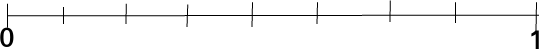
\includegraphics[width=.4\textwidth]{./pictures/7_7.png}
  \caption{}
  \label{fig:77}
\end{figure}

Отрезок разбивается на $n$ одинаковых частей (рис. \ref{fig:77}).

Это похоже на интегральные функции, то есть берётся значение и умножается на приращение.

Если бы винеровский процесс был дифференцируем, то это было бы равно
\begin{equation*}
  \int \limits_0^1 W \left( t \right) dW \left( t \right) =
  \frac{W^2 \left( 1 \right) }{2}.
\end{equation*}

Возьмём разность двух пределов
\begin{equation*}
  B_n - A_n =
  \sum \limits_{k = 0}^{n - 1}
    \left[ W \left( \frac{k + 1}{n} \right) - W \left( \frac{k}{n} \right) \right] \to
  1.
\end{equation*}
Получили длину отрезка.

Возьмём сумму двух пределов
\begin{equation*}
  B_n + A_n =
  \sum \limits_{k = 0}^{n - 1}
    \left[ W^2 \left( \frac{k + 1}{n} \right) - W^2 \left( \frac{k}{b} \right) \right] =
  W^2 \left( 1 \right).
\end{equation*}

То есть
\begin{equation*}
  A_n \to \frac{1}{2} \cdot W^2 \left( 1 \right) - \frac{1}{2}, \,
  B_n \to \frac{1}{2} \cdot W^2 \left( 1 \right) + \frac{1}{2}.
\end{equation*}

\subsubsection*{7.8}

\textit{Задание.}
Докажите, что сумма квадратов приращений винеровского процесса,
который соответствует разбиению $a = t_0 < t_1 < \dotsc < t_n = b$ отрезка $ \left[ a, b \right] $,
сходится к $b - a$ в среднем квадратическом при измельчении разбиения:
\begin{equation*}
  L_2 - \lim
    \sum \limits_{i = 0}^{n - 1}
      \left[ W \left( t_{i + 1} \right) - W \left( t_i \right) \right]^2 =
  b - a
\end{equation*}
при $ \max \left( t_{i + 1} - t_i \right) \to 0$.

\textit{Решение.}
Отрезок разбивается на конечное число отрезков
\begin{equation*}
  a = t_0 < t_1 < \dotsc < t_n = b,
\end{equation*}
и по этим отрезкам считается
\begin{equation*}
  \sum \limits_{i = 0}^{n - 1}
    \left[ W \left( t_{i + 1} \right) - W \left( t_i \right) \right]^2.
\end{equation*}
Надо проверить, что такие выражения сходится к $b - a$, то есть к длине отрезка, то есть
\begin{equation*}
  M \left\{
    \sum \limits_{i = 0}^{n - 1}
      \left[ W \left( t_{i + 1} \right) - W \left( t_i \right) \right]^2 - \left( b - a \right)
  \right\}^2 \to 0,
\end{equation*}
когда $ \max \left( t_{i + 1} - t_i \right) \to 0$.

Распределение разности
$W \left( t_{i + 1} \right) - W \left( t_i \right) \sim
  N \left( 0, t_{i + 1} - t_i \right) $,
то есть
\begin{equation*}
  M \left[ W \left( t_{i + 1} \right) - W \left( t_i \right) \right]^2 =
  t_{i + 1} - t_i,
\end{equation*}
то есть математическое ожидание всей этой суммы~---~это $b - a$, тогда
\begin{equation*}
  M \left[
    \sum \limits_{i = 0}^{n - 1}
      \left[ W \left( t_{i + 1} \right) - W \left( t_i \right) \right]^2 -
    \left( b - a \right) \right]^2 =
  D \sum \limits_{i = 0}^{n - 1}
    \left[ W \left( t_{i + 1} \right) - W \left( t_i \right) \right]^2 =
\end{equation*}
Разности независимы, значит и их квадраты независимы
\begin{equation*}
  = \sum \limits_{i = 0}^{n - 1}
    D \left[ W \left( t_{i + 1} \right) - W \left( t_i \right) \right]^2 =
\end{equation*}
То, что осталось,~---~это дисперсия квадрата случайной величины.
Обозначим $ \xi \sim N \left( 0, \sigma^2 \right) $,
тогда $D \xi^2 = M \xi^4 - \left( m \xi^2 \right)^2 = 3 \sigma^4 - \sigma^4 = 2 \sigma^4$.
Тогда
\begin{equation*}
= \sum \limits_{i = 0}^{n - 1} 2 \left( t_{i + 1} - t_i \right)^2 =
\end{equation*}
Один из множителей заменяем на максимальным в каждом слагаемом, максимум выносим
\begin{equation*}
  = 2 \max \left( t_{i + 1} - t_i \right)
  \sum \limits_{i = 0}^{n - 1} \left( t_{i + 1} - t_i \right) =
\end{equation*}
Сумма равна длине отрезка
\begin{equation*}
  = 2 \left( b - a \right) \max \left( t_{i + 1}, t_i \right) \to
  0.
\end{equation*}

Это называется квадратическая вариация винеровского процесса.

\addcontentsline{toc}{section}{Домашнее задание}
\section*{Домашнее задание}

\subsubsection*{7.10}

\textit{Задание.}
Для винеровского процесса вычислите:
\begin{enumerate}[label=\alph*)]
  \item $$cov \left(
      W \left( 2 \right), \int \limits_0^4 W \left( s \right) ds + W \left( 3 \right) \right);$$
  \item $$cov \left(
      W \left( 3 \right) + 2 W \left( 1 \right), \int \limits_1^3 W \left( s \right) ds \right).$$
\end{enumerate}

\textit{Решение.}
\begin{enumerate}[label=\alph*)]
  \item \begin{gather*}
    cov \left(
      W \left( 2 \right), \int \limits_0^4 W \left( s \right) ds + W \left( 3 \right) \right) = \\
    = cov \left[ W \left(2 \right), \int \limits_0^4 W \left( s \right) ds \right] +
    cov \left[ W \left( 2 \right), W \left( 3 \right) \right] = \\
    = \int \limits_0^4 cov \left[ W \left( 2 \right), W \left( s \right) \right] ds +
    \min \left( 2, 3 \right) =
    \int \limits_0^4 \min \left( 2, s \right) ds + \min \left( 2, 3 \right) = \\
    = \int \limits_0^2 \min \left( 2, s \right) ds + \int \limits_2^4 \min \left( 2, s \right) ds +
    2 =
    \int \limits_0^2 sds + \int \limits_2^4 2ds + 2 = \\
    = \left. \frac{s^2}{2} \right|_0^2 + \left. 2s \right|_2^4 + 2 =
    \frac{4}{2} + 2 \cdot 4 - 2 \cdot 2 + 2 =
    2 + 8 - 4 + 2 =
    8;
  \end{gather*}
  \item посчитаем
  \begin{gather*}
    cov \left(
      W \left( 3 \right) + 2 W \left( 1 \right), \int \limits_1^3 W \left( s \right) ds \right) = \\
    = cov \left[ W \left( 3 \right), \int \limits_1^3 W \left( s \right) ds \right] +
    cov \left[ 2W \left( 1 \right), \int \limits_1^3 W \left( s \right) ds \right] = \\
    = \int \limits_1^3 cov \left[ W \left( 3 \right), W \left( s \right) \right] ds +
    2 \int \limits_1^3 cov \left[ W \left( 1 \right), W \left( s \right) \right] ds = \\
    = \int \limits_1^3 \min \left( 3, s \right) ds +
    2 \int \limits_1^3 \min \left( 1, s \right) ds =
    \int \limits_1^3 sds + 2 \int \limits_1^3 ds =
    \left. \frac{s^2}{2} \right|_1^3 + \left. 2s \right|_1^3 = \\
    = \frac{9}{2} - \frac{1}{2} + 6 - 2 =
    \frac{8}{2} + 4 =
    4 + 4 =
    8.
  \end{gather*}
\end{enumerate}

\subsubsection*{7.11}

\textit{Задание.}
Пусть $ \tau \geq 0$ --- случайная величина,
которая имеет положительную непрерывную плотность распределения,
и пусть $X \left( t \right) = \mathbbm{1} \left\{ t \geq \tau \right\} $ --- процесс ожидания,
связанный с $ \tau $.
Докажите, что $ \left\{ X \left( t \right), \, t \in \left[ 0, 1 \right] \right\} $
не дифференцируем в среднем квадратическом.

\textit{Решение.}
Допустим, что процесс ожидания дифференцируем в среднем квадратическом.
Это означает, что для произвольного $t \in \left[ 0, 1 \right] $
существовала бы такая случайная величина $X' \left( t \right) $, что
$$M \left| \frac{X \left( t + h \right) - X \left( t \right) }{h} - X' \left( t \right) \right|^2 \to
  0, \,
  h \to 0.$$

Если бы такой предел существовал, то величина
$$M \left| \frac{X \left( t + h \right) - X \left( t \right) }{h} \right|^2$$
должна была бы быть ограниченной при $h \to 0$.
Но непосредственным вычислением показываем, что
$$M \left| \frac{X \left( t + h \right) - X \left( t \right) }{h} \right|^2 =
  M \left|
    \frac{ \mathbbm{1} \left\{ t + h \geq \tau \right\} - \mathbbm{1} \left\{ t \geq \tau \right\} }{h}
  \right|^2 =$$
Возводим в квадрат
$$= \frac{1}{h^2} \cdot M \left[
    \left( \mathbbm{1} \left\{ t + h \geq \tau \right\} \right)^2 -
    2 \cdot \mathbbm{1} \left\{ t + h \geq \tau \right\} \mathbbm{1} \left\{ t \geq \tau \right\} +
    \left( \mathbbm{1} \left\{ t \geq \tau \right\} \right)^2
  \right] =$$
Произведение индикаторов событий --- это индикатор пересечения этих событий
$$= \frac{1}{h^2} \cdot \left[
    M \mathbbm{1} \left\{ t + h \geq \tau \right\} -
    2M \mathbbm{1} \left\{
      \left\{ t + h \geq \tau \right\} \cap \left\{ t \geq \tau \right\} \right\} +
    M \mathbbm{1} \left\{ t \geq \tau \right\} \right] =$$
Математическое ожидание индикатора события --- это вероятность этого события
$$= \frac{1}{h^2} \cdot \left[
    P \left( t + h \geq \tau \right) - 2P \left( t + h \geq \tau \right) +
    P \left( t \geq \tau \right) \right] =$$
Приведём подобные
$$= \frac{1}{h^2} \cdot
  \left[ -P \left( t + h \geq \tau \right) + P \left( t \geq \tau \right) \right] =
  \frac{1}{h^2} \cdot
  \left[ P \left( \tau \leq t \right) - P \left( \tau \leq t + h \right) \right] =$$
Запишем через интеграл от плотности
$$= \frac{1}{h^2} \int \limits_t^{t + h} \tau \left( x \right) p_{ \tau } \left( x \right) dx \to
  \infty, \,
  h \to 0.$$

Это противоречие доказывает недифференцируемость в среднем квадратическом процесса ожидания.

\subsubsection*{7.12}

\textit{Задание.}
Пусть $ \xi $ --- дифференцируемый в среднем квадратическом процесс,
$f \in C^1 \left( \mathbb{R} \right) $ --- детерминированная функция.
Докажите,
что процесс $ \left\{ f \left( t \right) \xi \left( t \right), \, t \in \mathbb{R} \right\} $
имеет производную в среднем квадратическом и найдите её.

\textit{Решение.}
Нужно проверить, что
$$ \left \Vert
    \frac{f \left( t \right) \xi \left( t \right) - f \left( t_0 \right) \xi \left( t_0 \right) }{t - t_0} -
    f' \left( t_0 \right) \xi \left( t_0 \right) - f \left( t_0 \right) \xi' \left( t_0 \right)
  \right \Vert \to
  0,$$
когда $t \to t_0$.

Будем это проверять
$$M \left|
    \frac{f \left( t \right) \xi \left( t \right) - f \left( t_0 \right) \xi \left( t_0 \right) }{t - t_0} -
    f' \left( t_0 \right) \xi \left( t_0 \right) - f \left( t_0 \right) \xi' \left( t_0 \right)
  \right|^2 =$$
Поделим числитель на знаменатель
\begin{gather*}
  = M|
    \frac{f \left( t \right) \xi \left( t \right) }{t - t_0} -
    \frac{f \left( t_0 \right) \xi \left( t_0 \right) }{t - t_0} -
    \frac{f \left( t \right) \xi \left( t_0 \right) }{t - t_0} +
    \frac{f \left( t \right) \xi \left( t_0 \right) }{t - t_0} - \\
    - f' \left( t_0 \right) \xi \left( t_0 \right) - f \left( t_0 \right) \xi' \left( t_0 \right)
  |^2 = \\
  = M \left|
    f \left( t \right) \cdot \frac{ \xi \left( t \right) - \xi \left( t_0 \right) }{t - t_0} +
    \xi \left( t_0 \right) \cdot \frac{f \left( t \right) - f \left( t_0 \right) }{t - t_0} -
    f' \left( t_0 \right) \xi \left( t_0 \right) - f \left( t_0 \right) \xi' \left( t_0 \right)
  \right|^2 = \\
  = M \left|
    f \left( t \right) \xi' \left( t_0 \right) + \xi \left( t_0 \right) f' \left( t_0 \right) -
    f' \left( t_0 \right) \xi \left( t_0 \right) - f \left( t_0 \right) \xi' \left( t_0 \right)
  \right|^2 = \\
  = M \left|
    f \left( t \right) \xi' \left( t_0 \right) - f \left( t_0 \right) \xi' \left( t_0 \right)
  \right|^2 =
  M \left|
    \xi' \left( t_0 \right) \left[ f \left( t \right) - f \left( t_0 \right) \right]
  \right|^2 \to
  0
\end{gather*}
при $t \to t_0$.

\subsubsection*{7.13}

\textit{Задание.}
Пусть $ \eta $ --- решение задачи Коши
$$ \begin{cases}
    \eta' \left( t \right) = -\eta \left( t \right) + W \left( t \right), \\
    \eta \left( 0 \right) = 1.
  \end{cases}$$
Докажите, что
$$L_2-\lim \limits_{t \to +\infty } \frac{ \eta \left( t \right) }{t} =
  0.$$

\textit{Решение.}
Надо проверить, что
$$M \left[ \frac{ \eta \left( t \right) }{t} \right]^2 \to
  0$$
при $t \to +\infty $.

Из задачи 7.5 решением такой задачи Коши есть
$$ \eta \left( t \right) =
  e^{-t} + \int \limits_0^t e^{-\left( t - s \right) } W \left( s \right) ds.$$

Тогда
$$M \left[ \frac{ \eta \left( t \right) }{t} \right]^2 =
  M \left[
    \frac{e^{-t} + \int \limits_0^t e^{-\left( t - s \right) } W \left( s \right) ds}{t}
  \right]^2 =$$
Возведём в квадрат
$$= M \left\{
    \frac{e^{-2t}}{t^2} + \frac{2e^{-2t}}{t^2} \int \limits_0^t e^s W \left( s \right) ds +
    \frac{e^{-2t}}{t^2} \left[ \int \limits_0^t e^s W \left( s \right) ds \right]^2 \right\} =$$
Вынесем константу и внесём математическое ожидание
$$= \frac{e^{-2t}}{t^2} \left\{
    1 + \int \limits_0^t e^s MW \left( s \right) ds +
    M \left[ \int \limits_0^t e^s W \left( s \right) ds \right]^2 \right\} =$$
Математическое ожидание винеровского процесса равно нулю
\begin{gather*}
  = \frac{e^{-2t}}{t^2} \left[
    1 + \int \limits_0^t \int \limits_0^t e^{s_1 + s_2} \min \left( s_1, s_2 \right) ds_1 ds_2
  \right] = \\
  = \frac{e^{-2t}}{t^2} \left(
    1 + \int \limits_0^t \int \limits_{s_1}^t e^{s_1} e^{s_2} s_1 ds_1 ds_2 \right) =
  \frac{e^{-2t}}{t^2}
  \left( 1 + \int \limits_0^t e^{s_1} s_1 \left. e^{s_2} \right|_{s_1 }^t ds_1 \right) = \\
  = \frac{e^{-2t}}{t^2}
  \left[ 1 + \int \limits_0^t e^{s_1} s_1 \left( t - s_1 \right) ds_1 \right] = \\
  = \frac{e^{-2t}}{t^2}
  \left( 1 + t \int \limits_0^t e^{s_1} s_1 ds_1 - \int \limits_0^t e^{s_1} s_1^2 ds_1 \right) =
\end{gather*}
Оба интеграла берём по частям.
Для первого интеграла
$$u = s_1, \,
  dv = e^{s_1} ds_1, \,
  du = ds_1, \,
  v = \int \limits e^{s_1} ds_1 = e^{s_1}.$$
Для второго интеграла
$$u = s_1^2, \,
  dv = e^{s_1} ds_1, \,
  du = 2s_1 ds_1, \,
  v = e^{s_1}.$$
Тогда
$$= \frac{e^{-2t}}{t^2} \left(
    1 + \left. ts_1 e^{s_1} \right|_0^t - t \int \limits_0^t e^{s_1} ds_1 -
    \left. e^{s_1} s_1^2 \right|_0^t + 2 \int \limits_0^t e^{s_1} s_1 ds_1 \right) =$$
Подставим пределы интегрирования и возьмём интегралы
$$= \frac{e^{-2t}}{t^2} \left(
    1 + t^2 e^t - \left. te^{s_1} \right|_0^t - e^t t^2 + 2 \left. s_1 e^{s_1} \right|_0^t -
    2 \int \limits_0^t e^{s_1} ds_1 \right) =$$
Одинаковые слагаемые с разными знаками уничтожаются,
снова берём интеграл и подставляем пределы интегрирования
$$= \frac{e^{-2t}}{t^2} \left( 1 - te^t + t + 2te^t - 2 \left. e^{s_1} \right|_0^t \right) =
  \frac{e^{-2t}}{t^2} \left( 1 + te^t + t - 2e^t \right) =$$
Раскроем скобки
$$= \frac{e^{-2t}}{t^2} + \frac{e^{-3t}}{t} + \frac{e^{-2t}}{t} - \frac{2e^{-t}}{t^2} \approx
  -\frac{2e^{-2t}}{2t} - 3e^{-3t} - 2e^{-2t} + 2e^{-t} \approx$$
Снова используем правило Лопиталя
$$ \approx 2e^{-2t} - 3e^{-3t} - 2e^{-2t} + 2e^{-t} \to 0$$
при $t \to +\infty$.

\subsubsection*{7.14}

\textit{Задание.}
Докажите, что случайный процесс
$$ \eta \left( t \right) =
  \frac{1}{2} \cdot e^{-\lambda t} +
  \int \limits_0^t
    e^{-\lambda \left( t - s \right) } \left( \lambda m \left( s \right) +
    W \left( s \right) \right) ds, \,
  t \geq 0$$
является решением задачи Коши:
$$ \begin{cases}
    \eta' \left( t \right) =
    -\lambda \left( \eta \left( t \right) - m \left( t \right) \right) + W \left( t \right), \\
    \eta \left( 0 \right) = \frac{1}{2}.
  \end{cases}$$
Здесь $m \left( t \right) $ --- детерминированная функция.

\textit{Решение.}
$$ \eta \left( 0 \right) =
  \frac{1}{2} \cdot e^{-\lambda \cdot 0} +
  \int \limits_0^0
    e^{-\lambda \left( 0 -s \right) } \left[ \lambda m \left( s \right) + W \left( s \right) \right]
  ds =
  \frac{1}{2}.$$

Чтобы проверить, что уравнение выполняется, надо написать производную
\begin{gather*}
  \eta' \left( t \right) = \\
  = \frac{1}{2} \cdot \left( -\lambda \right) e^{-\lambda t} -
  \lambda e^{-\lambda t} \int \limits_0^t
    e^{ \lambda s} \left[ \lambda m \left( s \right) + W \left( s \right) \right] ds +
  e^{-\lambda \left( t - t \right) }
  \left[ \lambda m \left( t \right) + W \left( t \right) \right] = \\
  = -\lambda \left\{
    \frac{1}{2} \cdot e^{-\lambda t} -
    \int \limits_0^t
      e^{-\lambda \left( t - s \right) }
      \left[ \lambda m \left( s \right) + W \left( s \right) \right]
    ds - m \left( t \right)
  \right\} + W \left( t \right) = \\
  = -\lambda \left[ \eta \left( t \right) - m \left( t \right) \right] + W \left( t \right).
\end{gather*}
